
\begin{figure}
\centerline{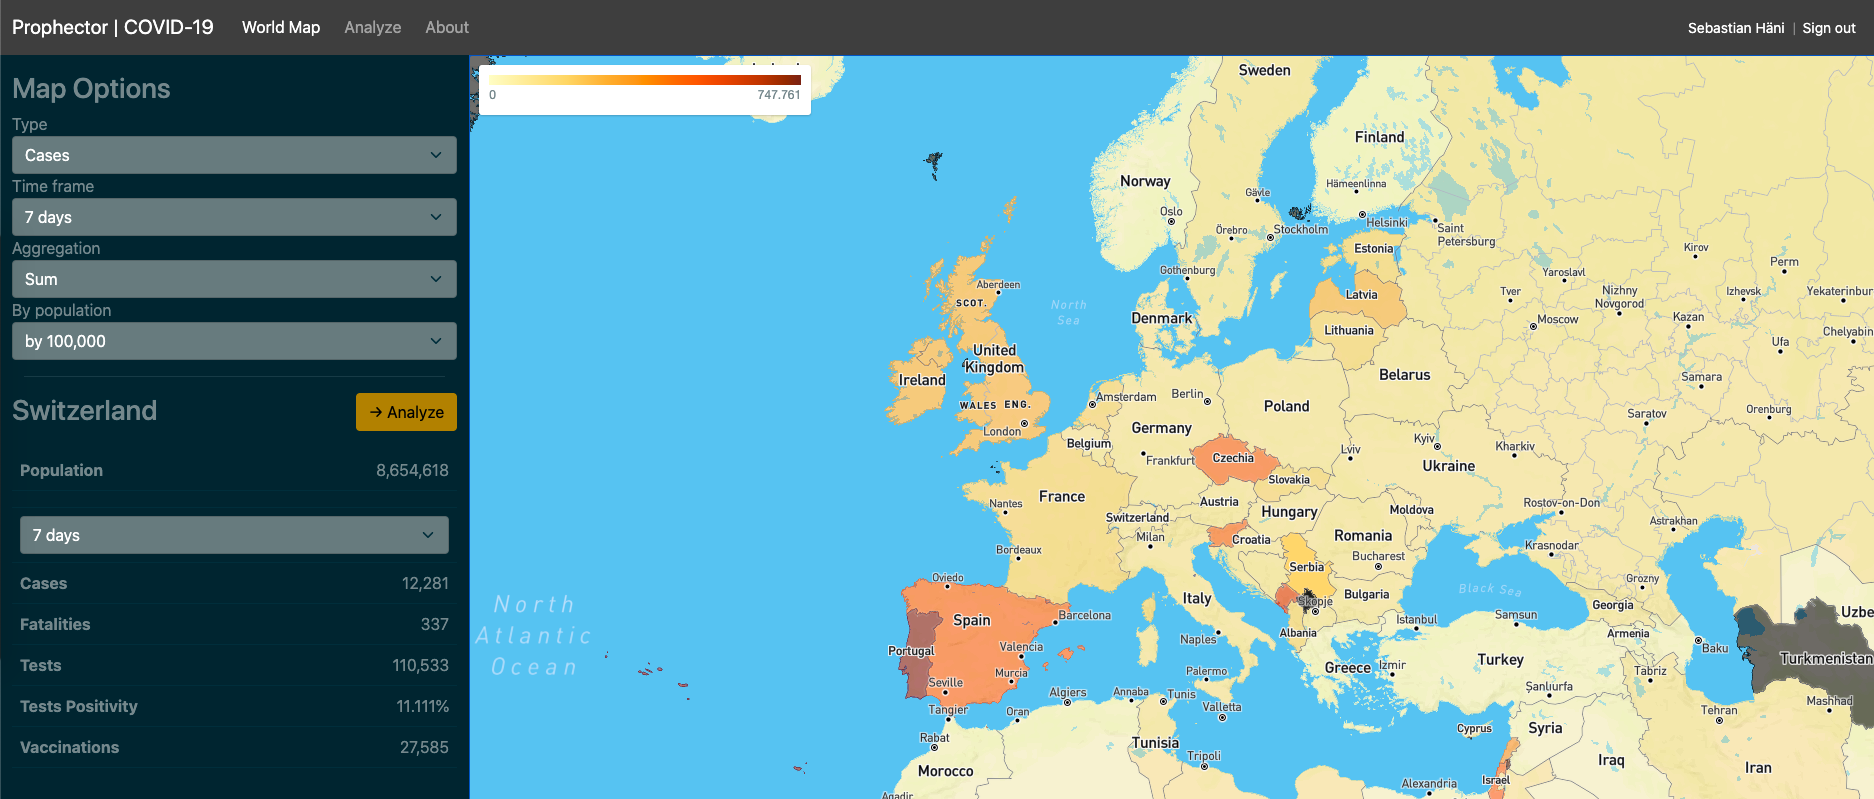
\includegraphics[scale=.135]{figs/screenshot-map.png}}
\caption{The screenshot shows the world map feature and the coloring of each country by cases summed in the last 7 days and normalized by the population factor. Currently Switzerland is selected.}
\label{fig:screenshot-map}
\end{figure}


\section{Visualizing COVID-19 data on a map}

The landing page of our web application is a world map visualizing the current state per country in a choropleth map as shown in figure \ref{fig:screenshot-map}. Each country receives a color on a scale of a statistical variable such as cases, tests, deaths, test positivity rate, or vaccinations within a time frame. The metric and aggregations can be changed individually by the user. This gives an overview and also an easy way to discover data as well as jump into a country's details.

With a map visualization come several challenges. The first one is the drawing of country polygons. Big and small countries should be discoverable while still being colored in according to our scale. The amount of polygon data is immense, and we didn't want to implement this ourselves. We used Mapbox\footnote{\href{https://www.mapbox.com}{https://www.mapbox.com}} which offers a JavaScript API to draw such maps. The maps are based on OpenStreetMap. The free tier of Mapbox includes 50,000 map loads per month.

The second challenge we encountered was preparing the data to visualize the map. Having just the raw time series in a database, we theoretically need to run aggregations for each country, which can involve querying thousands of data points. Since this data doesn't change over the course of minutes and rather over the course of a day, we added in-memory caching of the results in our backend. Once a new time window starts, the cache is invalidated and the first user accessing it, after it has been invalidated, has to wait roughly 10 seconds longer than the usual fast loading times, which was deemed acceptable by us (we actually pointed the health check to this URL, which means, it's likely that the health check triggers the refresh).

The third challenge is the color scale. Visualizing a map with all countries on a linear scale will skew visual inspections should there be an outlier in either direction. We decided to leave the scale linear as changing it to non-linear would also not be easy to recognize for a human, since a log scale is not easy to understand for a human. To generate a sequential color distribution over the linear scale, we used ColorBrewer\footnote{\href{https://colorbrewer2.org/\#type=sequential&scheme=YlOrRd&n=9}{https://colorbrewer2.org/\#type=sequential\&scheme=YlOrRd\&n=9}}. It contains several safe presets and directly gives a preview. The countries that have no data are colored in as black.

We added extra information to the map by providing helpful tooltips of the actual represented value as well as some additional information. Once the user clicks on a country, the country details appear, and the user is able to gather key metrics and can change the time frame for those interactively.
